\chapter{Fundamentação Teórica}
	\label{capituloReferencialTeorico}
	Neste trabalho de conclusão de curso, são usados alguns conceitos e técnicas da computação gráfica de forma adaptada ao objetivo proposto. Nas próximas seções são explicados os conceitos utilizados e suas respectivas aplicações no trabalho desenvolvido.
	
	\section{Projeções}
		\label{secaoProjecoes}
		
		Inicialmente, projeções são representações de objetos sob as restrições de um determinado ambiente. Em geometria analítica usam-se projeções para a descrição de vetores (as componentes do vetor são as projeções deste em cada uma das bases do sistema ordenado); no cotidiano, sombras geradas pelo nosso corpo no chão, por exemplo, é um caso específico de projeção (representação) do nosso corpo (obeto) na superfície plano do chão (ambiente) \cite{archiGeoBook}.
		
		Em computação gráfica, as projeções servem para representar objetos tridimensionais em dispositivos de visualização bidimensionais. Dependendo da utilização da visualização, diferentes formas de projetar o objeto tridimensional podem ser usadas \cite{archiGeoBook}; as duas principais são a projeção paralela e a projeção cônica.
		
		Independente do tipo de projeção, com apenas uma imagem não se pode estabelecer uma relação unívoca entre pontos no plano de projeção e pontos no espaço \cite{foto3D}. No entanto, relações de isometria (seção \ref{subsecaoProjecaoParalela}) ou proporcionalidade (seção \ref{subsecaoProjecaoConica}) podem incutir restrições aos pontos no espaço de forma a reduzir tal multiplicidade.
		
		\subsection{Projeção Paralela}
			\label{subsecaoProjecaoParalela}
			A projeção gráfica pode ser feita através de linhas paralelas entre si que ligam pontos do objeto ao plano de projeção (figura \ref{imagemProjecaoParalela}); esta projeção é chamada de projeção paralela \cite{archiGeoBook}. Neste caso, são mantidas as proporções entre as dimensões do objeto estudado (isometria) \cite{fundCompGraf}.
		
		\begin{figure}[!htb]
			\centering
			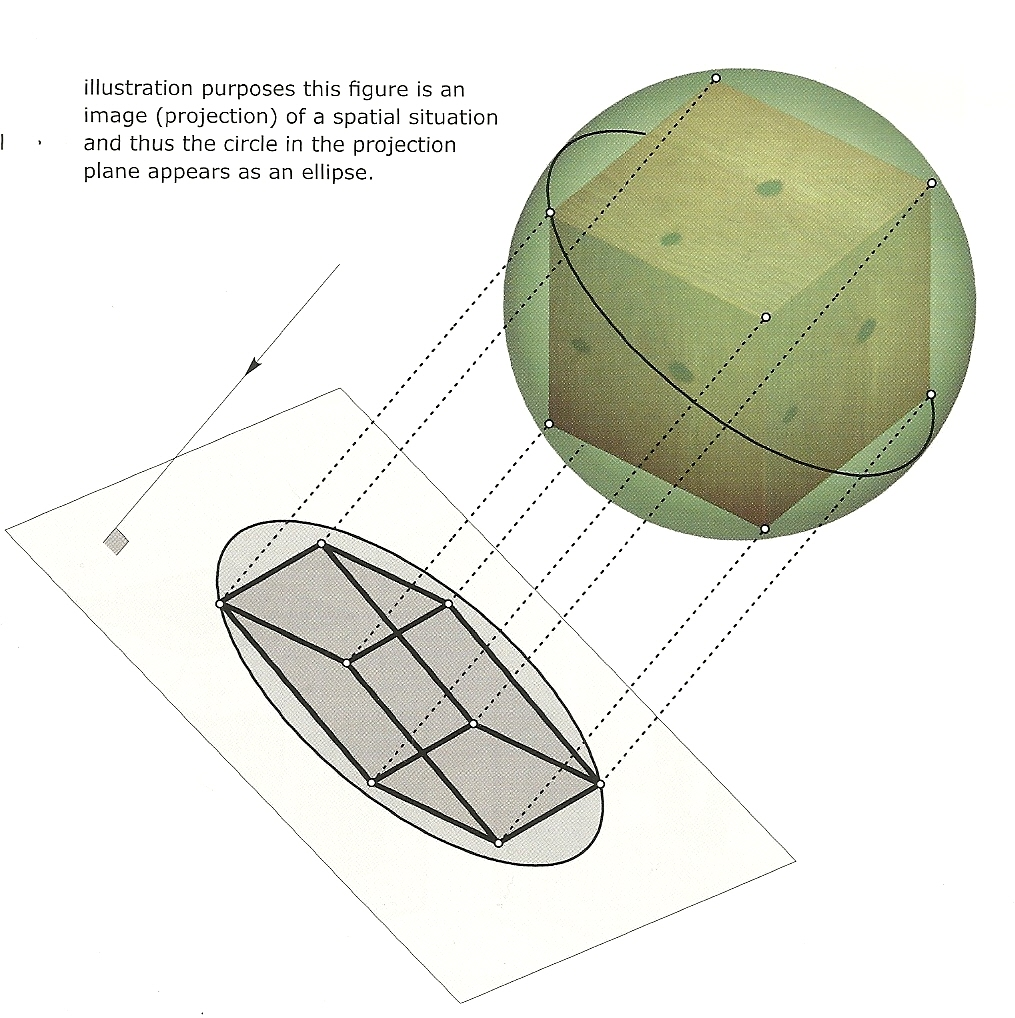
\includegraphics[height=5cm]{imagens/projecaoParalela.jpg}
			\caption{Projeção paralela em \cite{archiGeoBook}}
			\label{imagemProjecaoParalela}
		\end{figure}
		
			A isometria é uma característica interessante deste tipo de projeção pois a distância planar entre dois pontos é igual à sua distância no espaço.
			
			A transformação de um ponto 3D $P = (X_P, Y_P, Z_P)$ em um ponto 2D $P'$ sob a projeção paralela é dada pela equação \ref{formulaProjecaoParalela}, em coordenadas baseadas no Sistema de Coordenadas da Câmera \cite{foto3D}. Como pode-se notar, a projeção de $P$ independe da sua distância - $Z_P$ - ao plano de projeção e isto causa a multiplicidade projetiva.
			
			\begin{equation}
				\label{formulaProjecaoParalela}
				P' = (X_P, Y_P)
			\end{equation}
			
		\subsection{Projeção Cônica}
			\label{subsecaoProjecaoConica}
			Com o intuito de representar um objeto de forma similar à realidade, é aplicada a projeção cônica ou perspectiva \cite{archiGeoBook}. Tal projeção provoca uma deformação linear, proporcional à distância $Z_P$ ao plano de projeção, na posição planar do ponto $P = (X_P, Y_P, Z_P)$, que também está expresso em coordenadas do Sistema de Coordenadas da Câmera (equação \ref{formulaProjecaoConica}) \cite{foto3D}. Isto se dá pois a projeção $P'$ de $P$ é a interseção da reta que une o ponto 3D $e$ ao ponto $P$ (figura \ref{imagemProjecaoConica}), sendo $e$ o centro de projeção, que funciona de forma análoga ao olho de um observador humano \cite{archiGeoBook}.
			
			\begin{equation}
				\label{formulaProjecaoConica}
				P' = \left (\frac{X_P}{Z_P}, \frac{Y_P}{Z_P}\right )
			\end{equation}
			
			\begin{figure}[!htb]
				\centering
				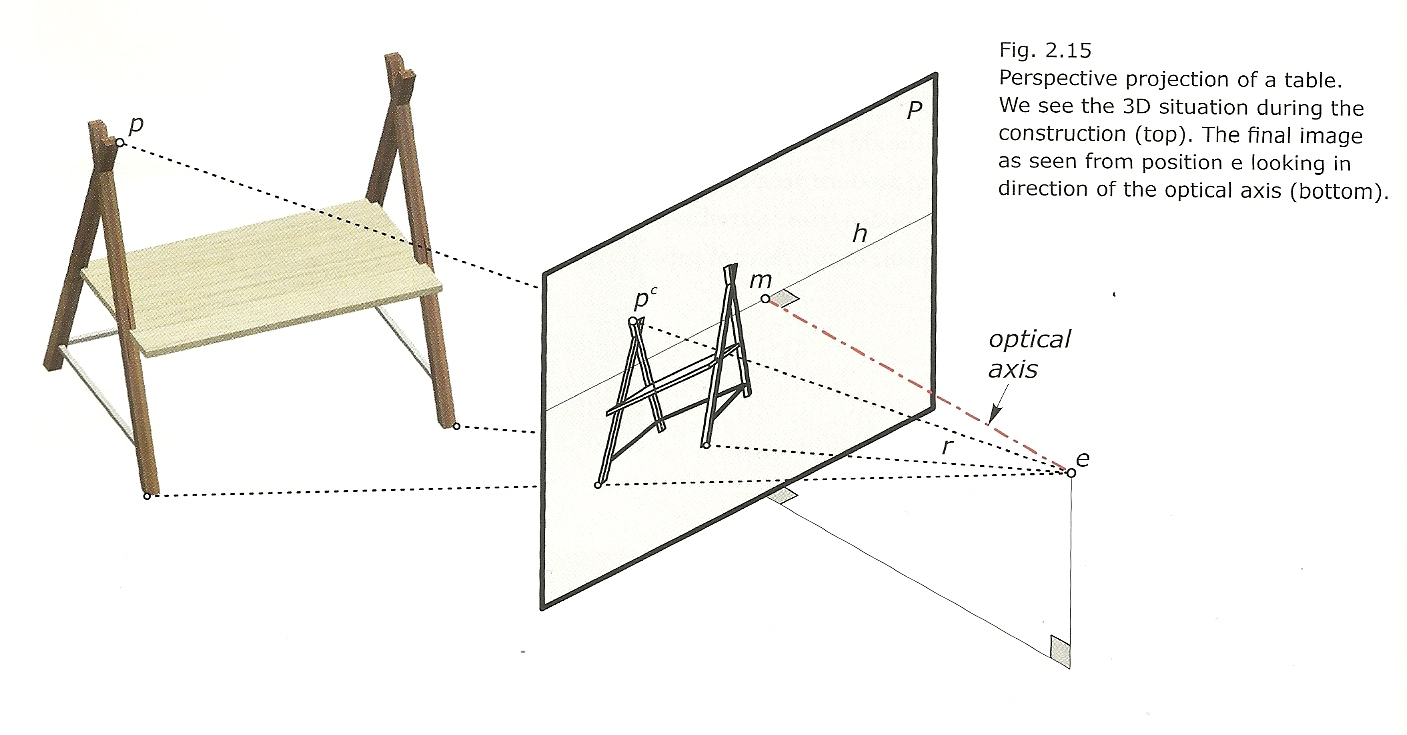
\includegraphics[height=5cm]{imagens/projecaoConica.jpg}
				\caption{Projeção cônica em \cite{archiGeoBook}}
				\label{imagemProjecaoConica}
			\end{figure}
			
			A deformação provocada pela projeção cônica impossibilita a existência da isometria, no entanto, com o processo de calibração de câmera virtual (seções \ref{secaoCamera} e \ref{secaoCalibracao}) é possível obter a distância entre dois pontos 3D pertencentes a um mesmo plano \cite{juizVirtual}.
	
	\section{Câmera Virtual}
		\label{secaoCamera}
	
		A operação básica de uma câmera virtual é a projeção \cite{fundCompGraf}. A fim de sintetizar uma imagem de um objeto digital com três dimensões, programas de visualização 3D implementam um modelo matemático que utiliza as técnicas discutidas anteriormente (seção \ref{secaoProjecoes}) para a transformação de 3D para 2D.
		
		Neste trabalho optou-se por desenvolver um modelo de câmera que projeta apenas em perspectiva dada a ausência, inicialmente, de bibliografia sobre modelos de câmeras de projeção paralela. No entanto, na seção \ref{secaoEstadoDaArteCalibracao} é exposta uma possibilidade de retificação desta limitação.
		
		Para um modelo altamente fiel à câmera real, devem ser feitas correções acerca de distorções de lentes \cite{animation} além de que uma câmera digital real, em termos geométricos, precisa converter as coordenadas de um objeto sob um sistema de referências global para um sistema de coordenadas em pixels passando por um sistema de coordenadas de câmera e de imagem, processo chamado de Transformações de Câmera \cite{foto3D}. Para este trabalho, não há distorção de lentes nas imagens (uma vez que são artificiais).
		
		Em \cite{foto3D} é descrita cada transformação entre cada sistema de coordenadas. No entanto, neste trabalho todas as transformações de câmera foram agrupadas, como em \cite{juizVirtual} e \cite{fundCompGraf}, uma vez que apenas interessa a transformação final e não os parâmetros explícitos da câmera. Assim, o modelo final de câmera $C$ utilizado foi o apresentado na equação \ref{formulaCamera}.
		
		\begin{equation}
			C = \begin{pmatrix}
						q_{1,1} & q_{1,2} & q_{1,3} & q_{1,4} \\
						q_{2,1} & q_{2,2} & q_{2,3} & q_{2,4} \\
						q_{3,1} & q_{3,2} & q_{3,3} & q_{3,4}
					\end{pmatrix}
			\label{formulaCamera}
		\end{equation}
		
		De forma que, aplicando $C$ a um ponto 3D, em coordenadas homogêneas \cite{fundCompGraf2} sob o Sistema de Coordenadas do Mundo \cite{foto3D}, obter-se-á diretamente o respectivo ponto 2D em termos de pixel na imagem.
	
	\section{Calibração de câmera}
		\label{secaoCalibracao}
	
		Costumeiramente, o modelo de câmera virtual é construído a partir dos parâmetros (intrínsecos e extrínsecos) \cite{fundCompGraf} da câmera, pode-se dizer que esta é a forma direta de especificação da câmera. 
		
		Neste trabalho, um dos empecilhos era o desconhecimento destes atributos da câmera e sem tal conhecimento não há como construir a transformação \ref{formulaCamera}. No entanto, com uma correspondência previamente conhecida entre pontos da imagem e pontos 3D, o modelo da câmera pode ser estimado; este processo é chamado de Calibração de Câmera (costuma-se chamar, também de \textit{Resectioning}, já que calibração pode envolver, ainda, ajuste cromático). \cite{juizVirtual}, \cite{szenbergDoutorado} e \cite{lectureCameraCalibration} aplicam apenas a calibração geométrica e usam o termo "Calibração".
		
		Como dito na seção \ref{secaoCamera}, a aplicação do modelo de câmera em pontos 3D $P = (X, Y, Z)$ leva a pontos 2D $P' = (u, v)$ da imagem; de forma que, segundo \cite{juizVirtual}, têm-se para cada correspondência de pontos 3D com 2D as equações \ref{formulaSistemaSimples1} e \ref{formulaSistemaSimples2}.
	
	\begin{equation}
		\label{formulaSistemaSimples1}
		u = \left(\frac{q_{1,1} . X + q_{1,2} . Y + q_{1,3} . Z + q_{1,4}}{q_{3,1} . X + q_{3,2} . Y + q_{3,3} . Z + q_{3,4}} \right)
	\end{equation}
	
	\begin{equation}
		\label{formulaSistemaSimples2}
		v = \left(\frac{q_{2,1} . X + q_{2,2} . Y + q_{2,3} . Z + q_{2,4}}{q_{3,1} . X + q_{3,2} . Y + q_{3,3} . Z + q_{3,4}} \right) 
	\end{equation}
	
	Como a matriz $C$ da câmera (equação \ref{formulaCamera}) tem 12 graus de liberdade, são necessários, no mínimo, 6 correspondências, com pontos 3D linearmente independentes, para que se monte um sistema $A^TA . Q = \lambda . Q$ dado por \ref{formulaSistemaMontado} possível de ser resolvido \cite{lectureCameraCalibration}.
	
	\begin{equation}
		\label{formulaSistemaMontado}
		\setcounter{MaxMatrixCols}{20}
		\begin{pmatrix}
			X_{1} & Y_{1} & Z_{1} & 1 & 0 & 0 & 0 & 0 & -u_{1}X_{1} & -u_{1}Y_{1} & -u_{1}Z_{1} & -u_{1} \\
			0 & 0 & 0 & 0 & X_{1} & Y_{1} & Z_{1} & 1 & -v_{1}X_{1} & -v_{1}Y_{1} & -v_{1}Z_{1} & -v_{1} \\
			\vdots & \vdots & \vdots & \vdots & \vdots & \vdots & \vdots & \vdots & \vdots & \vdots & \vdots & \vdots \\
			X_{n} & Y_{n} & Z_{n} & 1 & 0 & 0 & 0 & 0 & -u_{n}X_{n} & -u_{n}Y_{n} & -u_{n}Z_{n} & -u_{n} \\
			0 & 0 & 0 & 0 & X_{n} & Y_{n} & Z_{n} & 1 & -v_{n}X_{n} & -v_{n}Y_{n} & -v_{n}Z_{n} & -v_{n}	
		\end{pmatrix}
		.
		\begin{pmatrix}
			q_{1,1} \\
			q_{1,2} \\
			q_{1,3} \\
			q_{1,4} \\
			q_{2,1} \\
			q_{2,2} \\
			q_{2,3} \\
			q_{2,4} \\
			q_{3,1} \\
			q_{3,2} \\
			q_{3,3} \\
			q_{3,4} \\
		\end{pmatrix}
		=
		\begin{pmatrix}
			0 \\
			0 \\
			0 \\
			0 \\
			0 \\
			0 \\
			0 \\
			0 \\
			0 \\
			0 \\
			0 \\
			0 \\
		\end{pmatrix}
	\end{equation}
	
	O problema \ref{formulaSistemaMontado} é, costumeiramente, impreciso devido a erros na coleta dos valores dos pontos, neste trabalho, isto acontece devido a imprecisão do mouse ao demarcar pixels (vide capítulo \ref{capituloReconstrucao}). Assim, usa-se um aproximação pelo método dos mínimos quadrados.
	
	Pelo método dos mínimos quadrados, busca-se o menor valor para a matriz $C$ dada uma restrição que impeça se chegar à solução trivial ($C = 0$). Em \cite{juizVirtual} buscou-se uma restrição linear. No entanto, por trabalhar em coordenadas homogêneas, $C$ é independente de escala ($\lambda C \cong C$), podendo-se adotar a restrição $|C| = 1$ \cite{lectureCameraCalibration}.
	
	Por conseguinte, este é um problema de minimização solucionável por multiplicadores de Lagrange, onde se chega à expressão \ref{formulaMinimizacaoLagrange}. Observa-se que a solução $Q$ é um autovetor de $A^TA$ e, para a maior minimização, $Q$ deve ser o autovetor gerado pelo menor autovalor de $A^TA$. \cite{lectureLeastSquares}
	
	\begin{equation}
		\label{formulaMinimizacaoLagrange}
		A^TA . Q = \lambda . Q
	\end{equation}
	
	Por fim, a organização dos valores de $Q$ na forma de $C$ completa o processo de calibração da câmera, o que permite, a busca de pontos 3D correspondentes a pontos 2D da imagem (capítulo \ref{capituloReconstrucao}).
